\begin{comment}

\end{}
\label{chapter:metodo}
Este Capítulo descreve o método proposto neste trabalho, baseado em VHDL para analise de circuitos utilizando transformações de código e a ferramenta ESBMC.

\section{Visão geral do método}
O método consiste na análise de código VHDL de um circuito lógico através da ferramenta ESBMC. O método é apresentado na \autoref{fig:bpmn}, onde consiste inicialmente em um circuito lógico descrito em VHDL,com as assertivas a serem verificadas, posteriormente traduzida para linguagem C através de uma ferramenta chamada V2C. Após a tradução inicial, o código é reescrito, de modo que as assertivas presente no código VHDL sejam aceitas pelo ESBMC. Baseado nas assertivas o ESBMC analisa o código, de modo a verificar, caso em algum momento, uma das assertivas seja violada, caso ocorra, a mesma apresenta a assertiva violada.

\begin{figure}[htb]
	\begin{center}
    \caption{\label{fig:bpmn}Ciclo da ferramenta}
	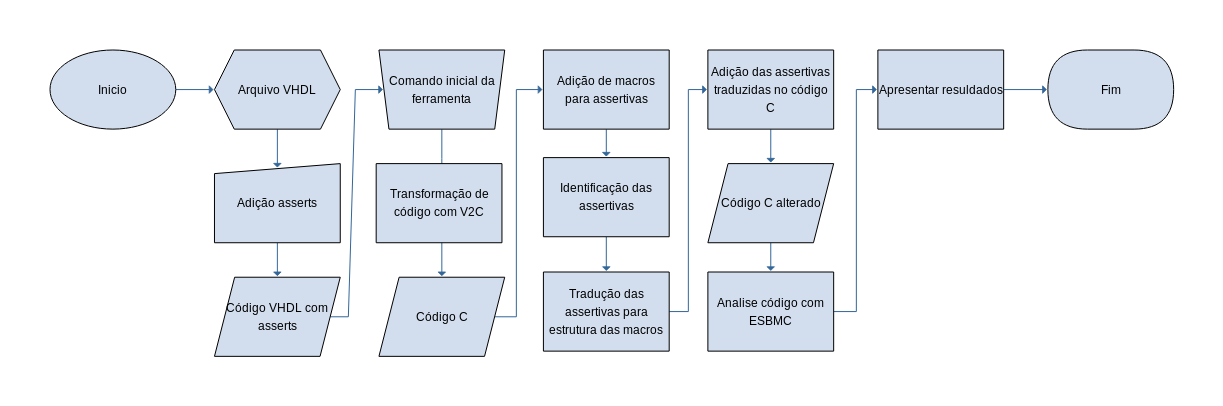
\includegraphics[scale=0.4]{Figuras/bpmn.png}
	\end{center}
    \legend{Fonte: Própria}
\end{figure}

\section{\label{cap:vhdl_assertivas}Código VHDL e assertivas}
\par
Na \autoref{fig:code_and} apresnta a estrutura geral do algoritmo na linguagem VHDL que será analisado pela ferramenta. O código não apresenta alteração na estrutura utilizada pela própria linguagem, composto de entidade e arquitetura. A utilização da linguagem é limitada apenas pela feramenta de tradução, V2C, que será apresentada na sessão \autoref{cap:traducao} e diferença no modo que assertiva será declarada, visto que a linguagem possui a utilização de assertivas nativamente.

\par
As assertivas, como citado anteriomente, apresenta estrutura diferente da utilizada pelo padrão do vhdl, as mesmas serão adicionadas ao código por meio das \textcolor{red}{tags} \textbf{@c2vhdl:ASSERT} e \textbf{@c2vhdl:END} e todo trecho de código entre estas \textcolor{red}{tags} deve esta comentado, desta forma não apresentará erro na execução do código em VHDL, caso o mesmo seja necessário. O trecho entre as \textcolor{red}{tags} apresentará trés informações necessárias:
\begin{enumerate}
\item \textbf{Condição:} A condição é a assertiva propriamente dita e que será analisado pela aplicação. A assertiva será precedida da palavra \textbf{assert} e/ou da palavra \textbf{not}, com isso a assertiva pode assumir propriedade negativa, conforme necessidade do usuário. A assertiva deve ser apresentada entre parenteses, conforme exemplificado na \autoref{fig:code_and}.
\item \textbf{Mensagem:} A mensagem é apresentada ao usuario, caso a assertiva falhe, pode ser indicando a propriedade violado, por exemplo ou quaquer outra mensagem a ser apresentada. E precedida pela palavra \textbf{report}.
\item \textbf{Gravidade:} O usuário pode um nível de gravidade, pode ser \textit{error} ou \textit{warning}. É precedido pela palavra \textbf{severity}.
\end{enumerate}

\begin{figure}[thp]
\caption{\label{fig:code_and} Exemplo de porta AND em VHDL com padrão da assertivas a ser adotada pelo método.}
	\begin{center}
    \begin{minipage}{0.6\textwidth}
    \begin{lstlisting}       
library ieee;
use ieee.std_logic_1164.all;

entity AND_ent is
port(   x, y: in bit;
        F: out bit
);
end AND_ent;

architecture behav1 of AND_ent is
begin
    --@c2vhdl:ASSERT
    --assert (x='__VERIFIER_nondet_int()' and y='__VERIFIER_nondet_int()')
    --report "Both values of signals x and y are equal to 1"
    --severity ERROR;
    --@c2vhdl:END
    
    process(x, y)
    begin
        if ((x='1') and (y='1')) then
            F <= '1';
        else
            F <= '0';
        end if;
    end process;
end behav1;

\end{lstlisting}
    \end{minipage}
	\end{center}
    \legend{Fonte: Própria.}
\end{figure}

\section{\label{cap:traducao}Tradução para código em linguagem C}
A tradução é utilizando a ferramenta V2c, e devido a ser uma ferramenta antiga a mesma apresenta certas limitação na tradução do código VHDL para ser, em outras palavras, a mesma não reconhece algumas estruturas especificas do VHDL. A ferramenta aceita apenas entradas e saídas do tipo: bit, std\underline{\space}ulogic, qsim\underline{\space}state, std\underline{\space}ulogic\underline{\space}vector e interger. Na parte de arquitetura, a ferramenta aceita uma gama maior de estruturas, operandos em expressoões do tipo: signal, variable, integers, strings e caracteres. Em expreções condicionais os operandos são AND, OR, NOT <=, =>,=,<,> e <>. Aceita também a estrutura de process, além da estutura block. A estrutura \textit{process} é limitada apenas a: if-else, case e  loops.

\par
Conforme especificado e seguindo os parametros da ferramenta, a mesma realiza a tradução, mantendo inalterado qualquer fragmento de código que esteja comentado, neste caso, qualquer assertiva existente no corpo do texto.
\section{Geraçao de código intermediário} 
\par
O código intrmediario é gerado a partir do código traduzido pelo V2C trabalhando diretamente nas assertivas comentadas no corpo do código. Devido as \textcolor{red}{tags} utilizadas e utilizando a tecnica de Regex, as assertivas são localizadas e traduzidas.

\par
A \autoref{fig:code_assert} apresenta um exemplo da assertiva em código VHDL, conforme explanado na sessão \autoref{cap:vhdl_assertivas}, a partir deste trecho a assertiva é inserida ao código para posteriomente ser analisada pelo ESBMC.

\begin{figure}[thp]
\caption{\label{fig:code_assert} Exemplo de assertiva seguindo o padrão proposto no método e apresentado na \autoref{fig:code_and}}. 
	\begin{center}
    \begin{minipage}{0.7\textwidth}
    \begin{lstlisting}       	
    --@c2vhdl:ASSERT
    --assert (x='__VERIFIER_nondet_int()' and y='__VERIFIER_nondet_int()')
    --report "Both values of signals x and y are equal to 1"
    --severity ERROR;
    --@c2vhdl:END
\end{lstlisting}
    \end{minipage}
	\end{center}
    \legend{Fonte: Própria.}
\end{figure}

\section{Analise ESBMC}
\end{comment}
